\documentclass{scrartcl}\usepackage[]{graphicx}\usepackage[]{color}
%% maxwidth is the original width if it is less than linewidth
%% otherwise use linewidth (to make sure the graphics do not exceed the margin)
\makeatletter
\def\maxwidth{ %
  \ifdim\Gin@nat@width>\linewidth
    \linewidth
  \else
    \Gin@nat@width
  \fi
}
\makeatother

\definecolor{fgcolor}{rgb}{0.345, 0.345, 0.345}
\newcommand{\hlnum}[1]{\textcolor[rgb]{0.686,0.059,0.569}{#1}}%
\newcommand{\hlstr}[1]{\textcolor[rgb]{0.192,0.494,0.8}{#1}}%
\newcommand{\hlcom}[1]{\textcolor[rgb]{0.678,0.584,0.686}{\textit{#1}}}%
\newcommand{\hlopt}[1]{\textcolor[rgb]{0,0,0}{#1}}%
\newcommand{\hlstd}[1]{\textcolor[rgb]{0.345,0.345,0.345}{#1}}%
\newcommand{\hlkwa}[1]{\textcolor[rgb]{0.161,0.373,0.58}{\textbf{#1}}}%
\newcommand{\hlkwb}[1]{\textcolor[rgb]{0.69,0.353,0.396}{#1}}%
\newcommand{\hlkwc}[1]{\textcolor[rgb]{0.333,0.667,0.333}{#1}}%
\newcommand{\hlkwd}[1]{\textcolor[rgb]{0.737,0.353,0.396}{\textbf{#1}}}%
\let\hlipl\hlkwb

\usepackage{framed}
\makeatletter
\newenvironment{kframe}{%
 \def\at@end@of@kframe{}%
 \ifinner\ifhmode%
  \def\at@end@of@kframe{\end{minipage}}%
  \begin{minipage}{\columnwidth}%
 \fi\fi%
 \def\FrameCommand##1{\hskip\@totalleftmargin \hskip-\fboxsep
 \colorbox{shadecolor}{##1}\hskip-\fboxsep
     % There is no \\@totalrightmargin, so:
     \hskip-\linewidth \hskip-\@totalleftmargin \hskip\columnwidth}%
 \MakeFramed {\advance\hsize-\width
   \@totalleftmargin\z@ \linewidth\hsize
   \@setminipage}}%
 {\par\unskip\endMakeFramed%
 \at@end@of@kframe}
\makeatother

\definecolor{shadecolor}{rgb}{.97, .97, .97}
\definecolor{messagecolor}{rgb}{0, 0, 0}
\definecolor{warningcolor}{rgb}{1, 0, 1}
\definecolor{errorcolor}{rgb}{1, 0, 0}
\newenvironment{knitrout}{}{} % an empty environment to be redefined in TeX

\usepackage{alltt}
\title{VR study script}
\subtitle{}
\date{\today}

% specify packages and configs
\usepackage{breakurl}
\def\UrlBreaks{\do\/\do-}
\usepackage{graphicx}
\usepackage{float}
\usepackage{natbib}
\usepackage{usebib}
\usepackage{lmodern}
\usepackage{slantsc}
\usepackage{amsmath}
\usepackage{amssymb}
\usepackage[utf8]{inputenc}
\usepackage{hyperref}
\hypersetup{colorlinks=true,
  linkcolor=black,
  citecolor=black,
  urlcolor=blue}
\IfFileExists{upquote.sty}{\usepackage{upquote}}{}
\begin{document}
\pagenumbering{gobble}
\maketitle
\newpage
\pagenumbering{arabic}

\section{R setup}
\label{sec:r-setup}

The first thing we do is set a random seed for R. This ensures we can
reproduce any analysis that has a random component.

\begin{knitrout}
\definecolor{shadecolor}{rgb}{0.969, 0.969, 0.969}\color{fgcolor}\begin{kframe}
\begin{alltt}
\hlstd{our_seed} \hlkwb{<-} \hlnum{123}
\hlkwd{set.seed}\hlstd{(our_seed)}
\end{alltt}
\end{kframe}
\end{knitrout}

We'll use `123' as our seed. Next we need to load the
libraries.

\begin{knitrout}
\definecolor{shadecolor}{rgb}{0.969, 0.969, 0.969}\color{fgcolor}\begin{kframe}
\begin{alltt}
\hlkwd{require}\hlstd{(knitr)}
\hlkwd{require}\hlstd{(lme4)}
\end{alltt}


{\ttfamily\noindent\itshape\color{messagecolor}{\#\# Loading required package: lme4}}

{\ttfamily\noindent\itshape\color{messagecolor}{\#\# Loading required package: Matrix}}

{\ttfamily\noindent\itshape\color{messagecolor}{\#\# Loading required package: methods}}\begin{alltt}
\hlkwd{require}\hlstd{(afex)}
\end{alltt}


{\ttfamily\noindent\itshape\color{messagecolor}{\#\# Loading required package: afex}}

{\ttfamily\noindent\itshape\color{messagecolor}{\#\# Loading required package: emmeans}}

{\ttfamily\noindent\itshape\color{messagecolor}{\#\# ************\\\#\# Welcome to afex. For support visit: http://afex.singmann.science/}}

{\ttfamily\noindent\itshape\color{messagecolor}{\#\# - Functions for ANOVAs: aov\_car(), aov\_ez(), and aov\_4()\\\#\# - Methods for calculating p-values with mixed(): 'KR', 'S', 'LRT', and 'PB'\\\#\# - 'afex\_aov' and 'mixed' objects can be passed to emmeans() for follow-up tests\\\#\# - Get and set global package options with: afex\_options()\\\#\# - Set orthogonal sum-to-zero contrasts globally: set\_sum\_contrasts()\\\#\# - For example analyses see: browseVignettes("{}afex"{})\\\#\# ************}}

{\ttfamily\noindent\itshape\color{messagecolor}{\#\# \\\#\# Attaching package: 'afex'}}

{\ttfamily\noindent\itshape\color{messagecolor}{\#\# The following object is masked from 'package:lme4':\\\#\# \\\#\#\ \ \ \  lmer}}\begin{alltt}
\hlkwd{require}\hlstd{(cowplot)}
\end{alltt}


{\ttfamily\noindent\itshape\color{messagecolor}{\#\# Loading required package: cowplot}}

{\ttfamily\noindent\itshape\color{messagecolor}{\#\# Loading required package: ggplot2}}

{\ttfamily\noindent\itshape\color{messagecolor}{\#\# \\\#\# Attaching package: 'cowplot'}}

{\ttfamily\noindent\itshape\color{messagecolor}{\#\# The following object is masked from 'package:ggplot2':\\\#\# \\\#\#\ \ \ \  ggsave}}\begin{alltt}
\hlkwd{require}\hlstd{(DHARMa)}
\end{alltt}


{\ttfamily\noindent\itshape\color{messagecolor}{\#\# Loading required package: DHARMa}}\begin{alltt}
\hlkwd{require}\hlstd{(xtable)}
\end{alltt}


{\ttfamily\noindent\itshape\color{messagecolor}{\#\# Loading required package: xtable}}\begin{alltt}
\hlkwd{require}\hlstd{(rockchalk)}
\end{alltt}


{\ttfamily\noindent\itshape\color{messagecolor}{\#\# Loading required package: rockchalk}}\begin{alltt}
\hlkwd{require}\hlstd{(tikzDevice)}
\end{alltt}


{\ttfamily\noindent\itshape\color{messagecolor}{\#\# Loading required package: tikzDevice}}\begin{alltt}
\hlkwd{require}\hlstd{(parallel)}
\end{alltt}


{\ttfamily\noindent\itshape\color{messagecolor}{\#\# Loading required package: parallel}}\begin{alltt}
\hlkwd{require}\hlstd{(fifer)}
\end{alltt}


{\ttfamily\noindent\itshape\color{messagecolor}{\#\# Loading required package: fifer}}

{\ttfamily\noindent\itshape\color{messagecolor}{\#\# Loading required package: MASS}}

{\ttfamily\noindent\itshape\color{messagecolor}{\#\# \\\#\# Attaching package: 'MASS'}}

{\ttfamily\noindent\itshape\color{messagecolor}{\#\# The following object is masked from 'package:rockchalk':\\\#\# \\\#\#\ \ \ \  mvrnorm}}\begin{alltt}
\hlkwd{require}\hlstd{(multcomp)}
\end{alltt}


{\ttfamily\noindent\itshape\color{messagecolor}{\#\# Loading required package: multcomp}}

{\ttfamily\noindent\itshape\color{messagecolor}{\#\# Loading required package: mvtnorm}}

{\ttfamily\noindent\itshape\color{messagecolor}{\#\# Loading required package: survival}}

{\ttfamily\noindent\itshape\color{messagecolor}{\#\# Loading required package: TH.data}}

{\ttfamily\noindent\itshape\color{messagecolor}{\#\# \\\#\# Attaching package: 'TH.data'}}

{\ttfamily\noindent\itshape\color{messagecolor}{\#\# The following object is masked from 'package:MASS':\\\#\# \\\#\#\ \ \ \  geyser}}\begin{alltt}
\hlkwd{require}\hlstd{(vcdExtra)}
\end{alltt}


{\ttfamily\noindent\itshape\color{messagecolor}{\#\# Loading required package: vcdExtra}}

{\ttfamily\noindent\itshape\color{messagecolor}{\#\# Loading required package: vcd}}

{\ttfamily\noindent\itshape\color{messagecolor}{\#\# Loading required package: grid}}

{\ttfamily\noindent\itshape\color{messagecolor}{\#\# Loading required package: gnm}}\end{kframe}
\end{knitrout}

\section{Reading the files}
\label{sec:read-data}
We now read in the data files.

\begin{knitrout}
\definecolor{shadecolor}{rgb}{0.969, 0.969, 0.969}\color{fgcolor}\begin{kframe}
\begin{alltt}
\hlstd{child.data} \hlkwb{<-} \hlkwd{read.csv}\hlstd{(}\hlstr{"vr_data/childrenCSV.csv"}\hlstd{)}
\hlstd{carsac.data} \hlkwb{<-} \hlkwd{read.csv}\hlstd{(}\hlstr{"vr_data/selfSacCSV.csv"}\hlstd{)}
\hlstd{sidewalk.data} \hlkwb{<-} \hlkwd{read.csv}\hlstd{(}\hlstr{"vr_data/sidewalkCSV.csv"}\hlstd{)}
\end{alltt}
\end{kframe}
\end{knitrout}

Some of the variables need cleaning, so we rename them.
\begin{knitrout}
\definecolor{shadecolor}{rgb}{0.969, 0.969, 0.969}\color{fgcolor}\begin{kframe}
\begin{alltt}
\hlcom{# rename gender variable}
\hlkwd{colnames}\hlstd{(child.data)[}\hlnum{2}\hlstd{]} \hlkwb{<-} \hlstr{"gender"}

\hlcom{# rename driver variable}
\hlkwd{colnames}\hlstd{(child.data)[}\hlnum{3}\hlstd{]} \hlkwb{<-} \hlstr{"motorist"}

\hlcom{# rename levels for driver}
\hlstd{child.data}\hlopt{$}\hlstd{motorist} \hlkwb{<-} \hlkwd{factor}\hlstd{(child.data}\hlopt{$}\hlstd{motorist,}
                            \hlkwc{levels} \hlstd{=} \hlkwd{c}\hlstd{(}\hlstr{"False"}\hlstd{,} \hlstr{"True"}\hlstd{),}
                            \hlkwc{labels} \hlstd{=} \hlkwd{c}\hlstd{(}\hlstr{"human"}\hlstd{,} \hlstr{"self-driving"}\hlstd{))}

\hlcom{# set participant to factor}
\hlstd{child.data}\hlopt{$}\hlstd{participant.ID} \hlkwb{<-} \hlkwd{factor}\hlstd{(child.data}\hlopt{$}\hlstd{participant.ID)}

\hlcom{# rename levels for gender}
\hlstd{child.data}\hlopt{$}\hlstd{gender} \hlkwb{<-} \hlkwd{factor}\hlstd{(child.data}\hlopt{$}\hlstd{gender,}
                            \hlkwc{levels} \hlstd{=} \hlkwd{c}\hlstd{(}\hlstr{"False"}\hlstd{,} \hlstr{"True"}\hlstd{),}
                            \hlkwc{labels} \hlstd{=} \hlkwd{c}\hlstd{(}\hlstr{"female"}\hlstd{,} \hlstr{"male"}\hlstd{))}

\hlcom{# remove sanity check and perception check failures}
\hlstd{child.sub} \hlkwb{<-} \hlkwd{subset}\hlstd{(child.data, child.data}\hlopt{$}\hlstd{passedSanCheck} \hlopt{==} \hlstr{"True"}\hlstd{)}
\hlstd{child.sub} \hlkwb{<-} \hlkwd{subset}\hlstd{(child.sub,} \hlopt{!}\hlstd{(child.sub}\hlopt{$}\hlstd{perceivedCar} \hlopt{==} \hlstr{"Mensch"} \hlopt{&}
                                 \hlstd{child.sub}\hlopt{$}\hlstd{motorist} \hlopt{==} \hlstr{"self-driving"}\hlstd{))}



\hlcom{# carsac}

\hlcom{# rename gender variable}
\hlkwd{colnames}\hlstd{(carsac.data)[}\hlnum{2}\hlstd{]} \hlkwb{<-} \hlstr{"gender"}

\hlcom{# rename driver variable}
\hlkwd{colnames}\hlstd{(carsac.data)[}\hlnum{3}\hlstd{]} \hlkwb{<-} \hlstr{"motorist"}

\hlcom{# rename levels for driver}
\hlstd{carsac.data}\hlopt{$}\hlstd{motorist} \hlkwb{<-} \hlkwd{factor}\hlstd{(carsac.data}\hlopt{$}\hlstd{motorist,}
                            \hlkwc{levels} \hlstd{=} \hlkwd{c}\hlstd{(}\hlstr{"False"}\hlstd{,} \hlstr{"True"}\hlstd{),}
                            \hlkwc{labels} \hlstd{=} \hlkwd{c}\hlstd{(}\hlstr{"human"}\hlstd{,} \hlstr{"self-driving"}\hlstd{))}

\hlstd{carsac.data}\hlopt{$}\hlstd{participant.ID} \hlkwb{<-} \hlkwd{factor}\hlstd{(carsac.data}\hlopt{$}\hlstd{participant.ID)}

\hlcom{# rename levels for gender}
\hlstd{carsac.data}\hlopt{$}\hlstd{gender} \hlkwb{<-} \hlkwd{factor}\hlstd{(carsac.data}\hlopt{$}\hlstd{gender,}
                            \hlkwc{levels} \hlstd{=} \hlkwd{c}\hlstd{(}\hlstr{"False"}\hlstd{,} \hlstr{"True"}\hlstd{),}
                            \hlkwc{labels} \hlstd{=} \hlkwd{c}\hlstd{(}\hlstr{"female"}\hlstd{,} \hlstr{"male"}\hlstd{))}

\hlstd{carsac.sub} \hlkwb{<-} \hlkwd{subset}\hlstd{(carsac.data, carsac.data}\hlopt{$}\hlstd{passedSanCheck} \hlopt{==} \hlstr{"True"}\hlstd{)}
\hlstd{carsac.sub} \hlkwb{<-} \hlkwd{subset}\hlstd{(carsac.sub,} \hlopt{!}\hlstd{(carsac.sub}\hlopt{$}\hlstd{perceivedCar} \hlopt{==} \hlstr{"Mensch"} \hlopt{&}
                                   \hlstd{carsac.sub}\hlopt{$}\hlstd{motorist} \hlopt{==} \hlstr{"self-driving"}\hlstd{))}



\hlcom{# sidewalk}

\hlcom{# rename gender variable}
\hlkwd{colnames}\hlstd{(sidewalk.data)[}\hlnum{2}\hlstd{]} \hlkwb{<-} \hlstr{"gender"}

\hlcom{# rename driver variable}
\hlkwd{colnames}\hlstd{(sidewalk.data)[}\hlnum{3}\hlstd{]} \hlkwb{<-} \hlstr{"motorist"}

\hlcom{# set participant to factor}
\hlstd{sidewalk.data}\hlopt{$}\hlstd{participant.ID} \hlkwb{<-} \hlkwd{factor}\hlstd{(sidewalk.data}\hlopt{$}\hlstd{participant.ID)}

\hlcom{# rename levels for driver}
\hlstd{sidewalk.data}\hlopt{$}\hlstd{motorist} \hlkwb{<-} \hlkwd{factor}\hlstd{(sidewalk.data}\hlopt{$}\hlstd{motorist,}
                            \hlkwc{levels} \hlstd{=} \hlkwd{c}\hlstd{(}\hlstr{"False"}\hlstd{,} \hlstr{"True"}\hlstd{),}
                            \hlkwc{labels} \hlstd{=} \hlkwd{c}\hlstd{(}\hlstr{"human"}\hlstd{,} \hlstr{"self-driving"}\hlstd{))}


\hlcom{# rename levels for gender}
\hlstd{sidewalk.data}\hlopt{$}\hlstd{gender} \hlkwb{<-} \hlkwd{factor}\hlstd{(sidewalk.data}\hlopt{$}\hlstd{gender,}
                            \hlkwc{levels} \hlstd{=} \hlkwd{c}\hlstd{(}\hlstr{"False"}\hlstd{,} \hlstr{"True"}\hlstd{),}
                            \hlkwc{labels} \hlstd{=} \hlkwd{c}\hlstd{(}\hlstr{"female"}\hlstd{,} \hlstr{"male"}\hlstd{))}

\hlcom{# sanity check}
\hlstd{sidewalk.sub} \hlkwb{<-} \hlkwd{subset}\hlstd{(sidewalk.data, sidewalk.data}\hlopt{$}\hlstd{passedSanCheck} \hlopt{==} \hlstr{"True"}\hlstd{)}
\hlstd{sidewalk.sub} \hlkwb{<-} \hlkwd{subset}\hlstd{(sidewalk.sub,} \hlopt{!}\hlstd{(sidewalk.sub}\hlopt{$}\hlstd{perceivedCar} \hlopt{==} \hlstr{"Mensch"} \hlopt{&}
                                       \hlstd{sidewalk.sub}\hlopt{$}\hlstd{motorist} \hlopt{==} \hlstr{"self-driving"}\hlstd{))}
\end{alltt}
\end{kframe}
\end{knitrout}

\section{Manipulation check}
\label{sec:manip-check}

We use a \(\chi^2\) goodness of fit test to see if perspective
affects identification.  First we create a subset of only one trial,
and collapse the two pedestrian perspectives.
\begin{knitrout}
\definecolor{shadecolor}{rgb}{0.969, 0.969, 0.969}\color{fgcolor}\begin{kframe}
\begin{alltt}
\hlstd{manip_check.sub} \hlkwb{<-} \hlkwd{subset}\hlstd{(child.sub, trial} \hlopt{==} \hlstr{"largeGroups"}\hlstd{)}

\hlstd{manip_check.sub}\hlopt{$}\hlstd{perspective} \hlkwb{<-} \hlkwd{combineLevels}\hlstd{(manip_check.sub}\hlopt{$}\hlstd{perspective,}
                                             \hlkwc{levs} \hlstd{=} \hlkwd{c}\hlstd{(}\hlstr{"PedLarge"}\hlstd{,} \hlstr{"PedSmall"}\hlstd{),}
                                             \hlkwc{newLabel} \hlstd{=} \hlkwd{c}\hlstd{(}\hlstr{"Pedestrian"}\hlstd{))}
\end{alltt}
\begin{verbatim}
## The original levels Observer Passenger PedLarge PedSmall 
## have been replaced by Observer Passenger Pedestrian
\end{verbatim}
\end{kframe}
\end{knitrout}

Next we create a contingency table.
\begin{kframe}
\begin{alltt}
\hlstd{manip_check.xtab} \hlkwb{<-} \hlkwd{xtabs}\hlstd{(}\hlopt{~}\hlstd{perspective} \hlopt{+} \hlstd{perceivedIden,} \hlkwc{data} \hlstd{= manip_check.sub)}
\hlkwd{print}\hlstd{(}\hlkwd{xtable}\hlstd{(manip_check.xtab))}
\end{alltt}
\end{kframe}% latex table generated in R 3.4.3 by xtable 1.8-2 package
% Wed Jan 24 19:31:49 2018
\begin{table}[ht]
\centering
\begin{tabular}{rrrr}
  \hline
 & Beobachter & Fußgänger & Mitfahrer \\ 
  \hline
Observer &  30 &   5 &  10 \\ 
  Passenger &   7 &   3 &  34 \\ 
  Pedestrian &  33 &  57 &   3 \\ 
   \hline
\end{tabular}
\end{table}


Then we compute the test statistic.
\begin{knitrout}
\definecolor{shadecolor}{rgb}{0.969, 0.969, 0.969}\color{fgcolor}\begin{kframe}
\begin{alltt}
\hlstd{manip_check.chisq} \hlkwb{<-} \hlkwd{chisq.test}\hlstd{(manip_check.xtab,} \hlkwc{simulate.p.value} \hlstd{=} \hlnum{TRUE}\hlstd{)}
\hlstd{manip_check.chisq}
\end{alltt}
\begin{verbatim}
## 
## 	Pearson's Chi-squared test with simulated p-value (based on 2000
## 	replicates)
## 
## data:  manip_check.xtab
## X-squared = 114.01, df = NA, p-value = 0.0004998
\end{verbatim}
\end{kframe}
\end{knitrout}

If the test statistic is significant, we perform follow-up comparisons.

\begin{kframe}
\begin{alltt}
\hlstd{alpha} \hlkwb{<-} \hlnum{0.05}
\hlkwa{if} \hlstd{(manip_check.chisq}\hlopt{$}\hlstd{p.value} \hlopt{<=} \hlstd{alpha)\{}
    \hlstd{manip_check.post} \hlkwb{<-} \hlkwd{chisq.post.hoc}\hlstd{(manip_check.xtab)}
    \hlstd{\}}
\end{alltt}
\end{kframe}Adjusted p-values used the fdr method.

\begin{kframe}\begin{alltt}
\hlkwd{print}\hlstd{(}\hlkwd{xtable}\hlstd{(manip_check.post))}
\end{alltt}
\end{kframe}% latex table generated in R 3.4.3 by xtable 1.8-2 package
% Wed Jan 24 19:31:50 2018
\begin{table}[ht]
\centering
\begin{tabular}{rlrr}
  \hline
 & comparison & raw.p & adj.p \\ 
  \hline
1 & Observer vs. Passenger & 0.00 & 0.00 \\ 
  2 & Observer vs. Pedestrian & 0.00 & 0.00 \\ 
  3 & Passenger vs. Pedestrian & 0.00 & 0.00 \\ 
   \hline
\end{tabular}
\end{table}


\section{Child vs adult dilemmas}
\label{sec:child}

\subsection{Visualising the raw responses}
\label{sec:child-raw}

First we look at the raw proportions of the responses.
\begin{knitrout}
\definecolor{shadecolor}{rgb}{0.969, 0.969, 0.969}\color{fgcolor}\begin{kframe}
\begin{alltt}
\hlstd{child.xtabs} \hlkwb{<-} \hlkwd{xtabs}\hlstd{(}\hlopt{~} \hlstd{motorist} \hlopt{+} \hlstd{perspective} \hlopt{+} \hlstd{decision,} \hlkwc{data} \hlstd{= child.sub)}
\hlstd{child.mosaic} \hlkwb{<-} \hlkwd{mosaic}\hlstd{(child.xtabs,}
                       \hlkwc{gp} \hlstd{=} \hlkwd{gpar}\hlstd{(}\hlkwc{fill} \hlstd{=} \hlkwd{c}\hlstd{(}\hlstr{"light gray"}\hlstd{,} \hlstr{"dark gray"}\hlstd{)))}
\end{alltt}
\end{kframe}
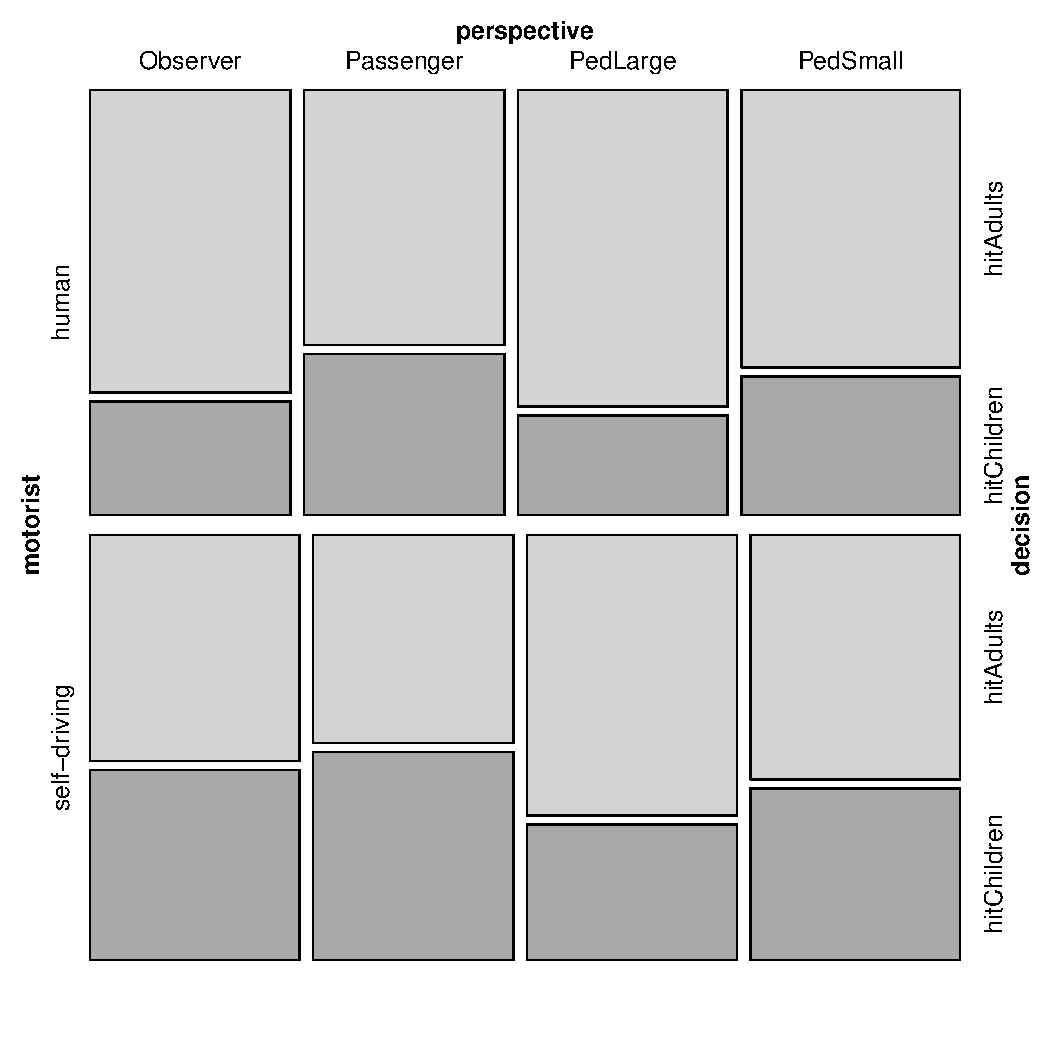
\includegraphics[width=\maxwidth]{figure/child-mosaic-1} 

\end{knitrout}

\subsection{The model}
\label{sec:child-model}

We run a logit mixed model to predict the decision of the participants.

\begin{kframe}
\begin{alltt}
\hlstd{(nc} \hlkwb{<-} \hlkwd{detectCores}\hlstd{())}
\end{alltt}
\end{kframe}[1] 12
\begin{kframe}\begin{alltt}
\hlstd{cl} \hlkwb{<-} \hlkwd{makeCluster}\hlstd{(}\hlkwd{rep}\hlstd{(}\hlstr{"localhost"}\hlstd{, nc))}

\hlstd{child_glmm} \hlkwb{<-} \hlkwd{mixed}\hlstd{(decision} \hlopt{~} \hlstd{perspective} \hlopt{+} \hlstd{motorist} \hlopt{+}
                        \hlstd{perspective}\hlopt{:}\hlstd{motorist} \hlopt{+}
                        \hlstd{trial} \hlopt{+} \hlstd{gender} \hlopt{+} \hlcom{#age +}
                        \hlstd{(}\hlnum{1} \hlopt{|} \hlstd{participant.ID),}
                    \hlkwc{method} \hlstd{=} \hlstr{"PB"}\hlstd{,} \hlcom{# change to PB for final}
                    \hlkwc{family} \hlstd{=} \hlstr{"binomial"}\hlstd{,} \hlkwc{data} \hlstd{= child.sub,}
                    \hlkwc{args_test} \hlstd{=} \hlkwd{list}\hlstd{(}\hlkwc{nsim} \hlstd{=} \hlnum{1000}\hlstd{,} \hlkwc{cl} \hlstd{= cl),} \hlkwc{cl} \hlstd{= cl,}
                    \hlkwc{control} \hlstd{=} \hlkwd{glmerControl}\hlstd{(}\hlkwc{optimizer} \hlstd{=} \hlstr{"bobyqa"}\hlstd{,}
                                           \hlkwc{optCtrl} \hlstd{=} \hlkwd{list}\hlstd{(}\hlkwc{maxfun} \hlstd{=} \hlnum{2e5}\hlstd{)))}
\end{alltt}


{\ttfamily\noindent\itshape\color{messagecolor}{\#\# Contrasts set to contr.sum for the following variables: decision, perspective, motorist, trial, gender, participant.ID}}\end{kframe}Fitting 6 (g)lmer() models.
Obtaining 5 p-values:
[.....]
\begin{kframe}\begin{alltt}
\hlkwd{stopCluster}\hlstd{(cl)}
\hlstd{child_glmm_anova} \hlkwb{<-} \hlstd{child_glmm}\hlopt{$}\hlstd{anova_table}
\hlkwd{print}\hlstd{(}\hlkwd{xtable}\hlstd{(child_glmm_anova))}
\end{alltt}
\end{kframe}% latex table generated in R 3.4.3 by xtable 1.8-2 package
% Wed Jan 24 19:42:45 2018
\begin{table}[ht]
\centering
\begin{tabular}{lrrrr}
  \hline
 & Chisq & Chi Df & Pr($>$Chisq) & Pr($>$PB) \\ 
  \hline
perspective & 3.90 & 3 & 0.2724 & 0.3986 \\ 
  motorist & 4.23 & 1 & 0.0398 & 0.0675 \\ 
  trial & 1.21 & 1 & 0.2713 & 0.2714 \\ 
  gender & 0.30 & 1 & 0.5820 & 0.6128 \\ 
  perspective:motorist & 0.45 & 3 & 0.9291 & 0.9328 \\ 
   \hline
\end{tabular}
\end{table}


We then check the residuals of the model.
\begin{knitrout}
\definecolor{shadecolor}{rgb}{0.969, 0.969, 0.969}\color{fgcolor}\begin{kframe}
\begin{alltt}
\hlstd{child_glmm.resid} \hlkwb{<-} \hlkwd{simulateResiduals}\hlstd{(}
    \hlkwc{fittedModel} \hlstd{= child_glmm}\hlopt{$}\hlstd{full_model,}
    \hlkwc{n} \hlstd{=} \hlnum{2000}\hlstd{)}
\hlstd{child_glmm_resid.plot} \hlkwb{<-} \hlkwd{plotSimulatedResiduals}\hlstd{(}
    \hlkwc{simulationOutput} \hlstd{= child_glmm.resid)}
\end{alltt}
\end{kframe}
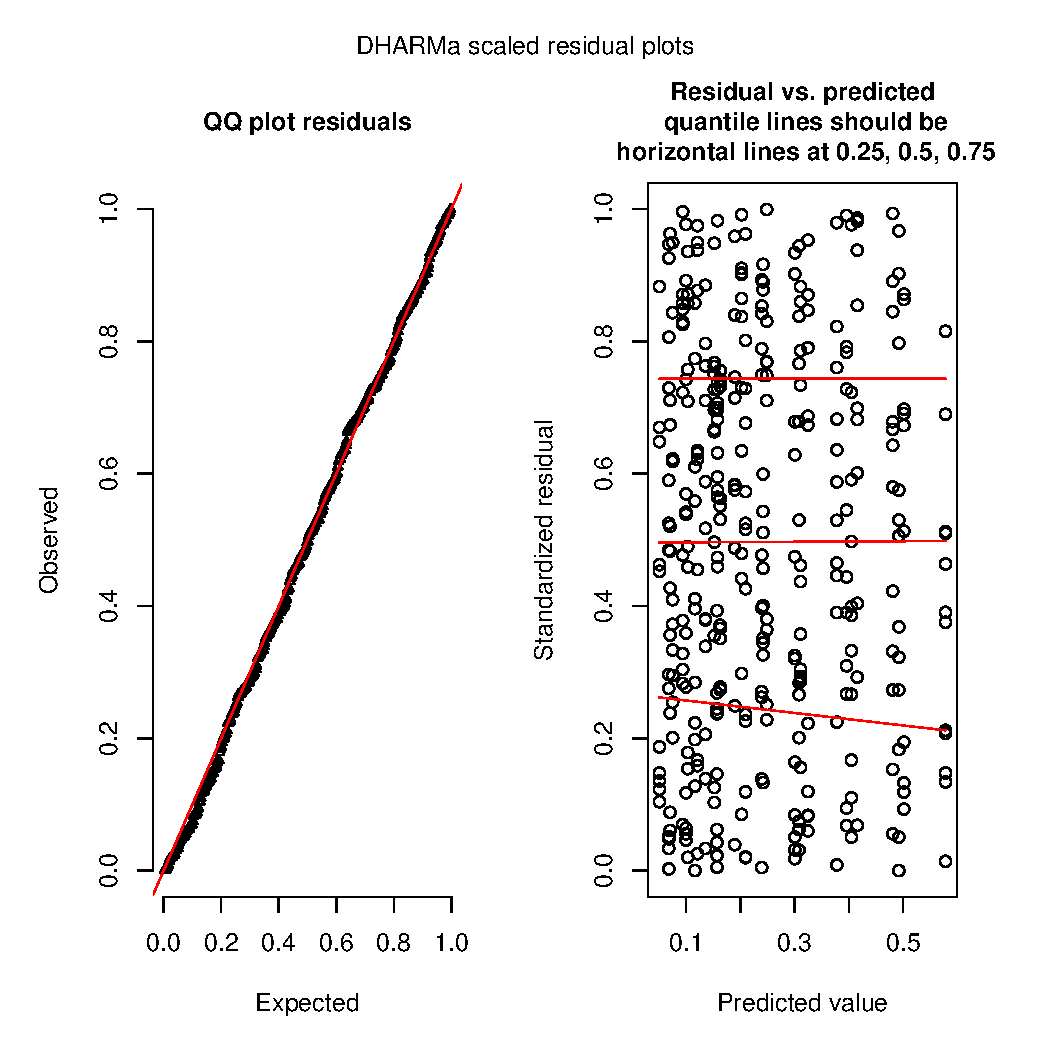
\includegraphics[width=\maxwidth]{figure/check-resid-1} 

\end{knitrout}

If they look okay, we follow up any significant differences.

\subsection{Plotting}
\label{sec:child-plot}


Depending on which effects or interactions we find, we probably want to change this plot. It currently just plots the Estimated Marginal Means for the 2-way interaction.

\begin{knitrout}
\definecolor{shadecolor}{rgb}{0.969, 0.969, 0.969}\color{fgcolor}\begin{kframe}
\begin{alltt}
\hlstd{child_emm_plot} \hlkwb{<-} \hlkwd{emmip}\hlstd{(child_glmm, perspective} \hlopt{~} \hlstd{trial} \hlopt{|} \hlstd{motorist,} \hlkwc{type} \hlstd{=} \hlstr{"response"}\hlstd{)} \hlopt{+}
    \hlkwd{theme_cowplot}\hlstd{(}\hlkwc{font_size} \hlstd{=} \hlnum{10}\hlstd{)} \hlopt{+}
    \hlkwd{scale_y_continuous}\hlstd{(}\hlkwc{name} \hlstd{=} \hlstr{"P(Choosing `crash car' as more acceptable)"}\hlstd{,}
                       \hlkwc{limits} \hlstd{=} \hlkwd{c}\hlstd{(}\hlnum{0}\hlstd{,} \hlnum{1}\hlstd{))} \hlopt{+} \hlkwd{coord_equal}\hlstd{(}\hlkwc{ratio} \hlstd{=} \hlnum{3}\hlstd{)} \hlopt{+}
    \hlkwd{scale_color_manual}\hlstd{(}\hlkwc{name} \hlstd{=} \hlstr{"Perspective"}\hlstd{,}
                       \hlkwc{labels} \hlstd{=} \hlkwd{c}\hlstd{(}\hlstr{"Bystander"}\hlstd{,}
                                  \hlstr{"Passenger"}\hlstd{,}
                                  \hlstr{"Pedestrian wAdults"}\hlstd{,}
                                  \hlstr{"Pedestrian wChildren"}\hlstd{),}
                       \hlkwc{values} \hlstd{=} \hlkwd{c}\hlstd{(}\hlstr{"red3"}\hlstd{,} \hlstr{"skyblue"}\hlstd{,} \hlstr{"orange1"}\hlstd{,} \hlstr{"purple"}\hlstd{))}
\hlstd{child_emm_plot}
\end{alltt}
\end{kframe}
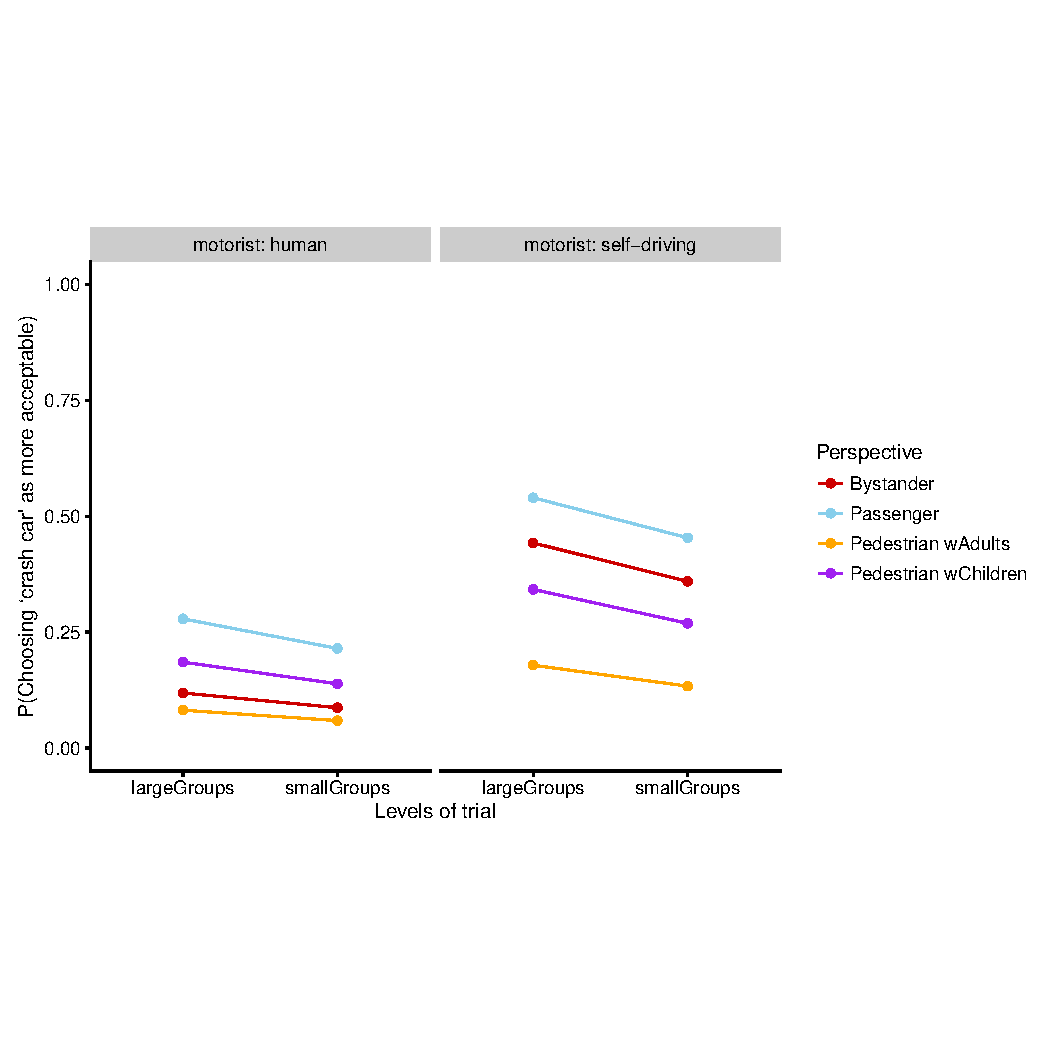
\includegraphics[width=\maxwidth]{figure/child-emm-plot-1} 

\end{knitrout}

\subsection{Follow-up comparisons}
For a good example, see https://osf.io/q2a3b/
\label{sec:child-followup}

If we find an interaction between perspective and motorist-type we
should follow that up with comparisons of perspective within each
level of motorist.

\begin{kframe}
\begin{alltt}
\hlstd{emm_child_i} \hlkwb{<-} \hlkwd{emmeans}\hlstd{(child_glmm,} \hlopt{~} \hlstd{perspective} \hlopt{|} \hlstd{motorist,} \hlkwc{type} \hlstd{=} \hlstr{"response"}\hlstd{,}
                       \hlkwc{contr} \hlstd{=} \hlstr{"pairwise"}\hlstd{)}
\hlkwd{xtable}\hlstd{(emm_child_i}\hlopt{$}\hlstd{contrasts)}
\end{alltt}
\end{kframe}% latex table generated in R 3.4.3 by xtable 1.8-2 package
% Wed Jan 24 19:42:50 2018
\begin{table}[ht]
\centering
\begin{tabular}{lrrrrl}
  \hline
contrast & odds.ratio & SE & df & z.ratio & p.value \\ 
  \hline
\multicolumn{6}{l}{motorist = human}\\
Observer / Passenger & 0.3479 & 0.4008 & Inf & -0.917 & 0.7960 \\ 
  Observer / PedLarge & 1.5163 & 1.7108 & Inf & 0.369 & 0.9829 \\ 
  Observer / PedSmall & 0.5917 & 0.6627 & Inf & -0.469 & 0.9659 \\ 
  Passenger / PedLarge & 4.3590 & 5.0289 & Inf & 1.276 & 0.5782 \\ 
  Passenger / PedSmall & 1.7009 & 1.9212 & Inf & 0.470 & 0.9656 \\ 
  PedLarge / PedSmall & 0.3902 & 0.4354 & Inf & -0.843 & 0.8337 \\ 
   \hline
\multicolumn{6}{l}{motorist = self-driving}\\
Observer / Passenger & 0.6760 & 0.7553 & Inf & -0.350 & 0.9852 \\ 
  Observer / PedLarge & 3.6493 & 4.0984 & Inf & 1.153 & 0.6568 \\ 
  Observer / PedSmall & 1.5251 & 1.6707 & Inf & 0.385 & 0.9806 \\ 
  Passenger / PedLarge & 5.3985 & 6.3213 & Inf & 1.440 & 0.4743 \\ 
  Passenger / PedSmall & 2.2562 & 2.5623 & Inf & 0.716 & 0.8906 \\ 
  PedLarge / PedSmall & 0.4179 & 0.4686 & Inf & -0.778 & 0.8644 \\ 
   \hline
\multicolumn{6}{l}{{\footnotesize Results are averaged over the levels of: trial, gender}}\\

\multicolumn{6}{l}{{\footnotesize P value adjustment: tukey method for comparing a family of 4 estimates}}\\

\multicolumn{6}{l}{{\footnotesize Tests are performed on the log odds ratio scale}}\\
\end{tabular}
\end{table}


If we find no interaction but a significant main effect of
perspective, we need to do follow-up multiple comparisons to find out
where the difference is.

\begin{kframe}
\begin{alltt}
\hlstd{emm_child_persp} \hlkwb{<-} \hlkwd{emmeans}\hlstd{(child_glmm, pairwise} \hlopt{~} \hlstd{perspective,}
                           \hlkwc{type} \hlstd{=} \hlstr{'response'}\hlstd{)}
\end{alltt}


{\ttfamily\noindent\itshape\color{messagecolor}{\#\# NOTE: Results may be misleading due to involvement in interactions}}\begin{alltt}
\hlkwd{xtable}\hlstd{(emm_child_persp}\hlopt{$}\hlstd{contrasts)}
\end{alltt}
\end{kframe}% latex table generated in R 3.4.3 by xtable 1.8-2 package
% Wed Jan 24 19:42:50 2018
\begin{table}[ht]
\centering
\begin{tabular}{lrrrrl}
  \hline
contrast & odds.ratio & SE & df & z.ratio & p.value \\ 
  \hline
Observer / Passenger & 0.4849 & 0.3907 & Inf & -0.898 & 0.8057 \\ 
  Observer / PedLarge & 2.3523 & 1.8836 & Inf & 1.068 & 0.7089 \\ 
  Observer / PedSmall & 0.9499 & 0.7427 & Inf & -0.066 & 0.9999 \\ 
  Passenger / PedLarge & 4.8510 & 4.0801 & Inf & 1.878 & 0.2377 \\ 
  Passenger / PedSmall & 1.9590 & 1.5768 & Inf & 0.835 & 0.8376 \\ 
  PedLarge / PedSmall & 0.4038 & 0.3218 & Inf & -1.138 & 0.6661 \\ 
   \hline
\multicolumn{6}{l}{{\footnotesize Results are averaged over the levels of: motorist, trial, gender}}\\

\multicolumn{6}{l}{{\footnotesize P value adjustment: tukey method for comparing a family of 4 estimates}}\\

\multicolumn{6}{l}{{\footnotesize Tests are performed on the log odds ratio scale}}\\
\end{tabular}
\end{table}


If we find a main effect of motorist-type, we need to calculate the
marginal means to see the effect.

\begin{kframe}
\begin{alltt}
\hlstd{emm_child_motorist} \hlkwb{<-} \hlkwd{emmeans}\hlstd{(child_glmm, pairwise} \hlopt{~} \hlstd{motorist,}
                              \hlkwc{type} \hlstd{=} \hlstr{'response'}\hlstd{)}
\end{alltt}


{\ttfamily\noindent\itshape\color{messagecolor}{\#\# NOTE: Results may be misleading due to involvement in interactions}}\begin{alltt}
\hlkwd{xtable}\hlstd{(emm_child_motorist}\hlopt{$}\hlstd{contrasts)}
\end{alltt}
\end{kframe}% latex table generated in R 3.4.3 by xtable 1.8-2 package
% Wed Jan 24 19:42:50 2018
\begin{table}[ht]
\centering
\begin{tabular}{lrrrrl}
  \hline
contrast & odds.ratio & SE & df & z.ratio & p.value \\ 
  \hline
human / self-driving & 0.3158 & 0.1869 & Inf & -1.948 & 0.0514 \\ 
   \hline
\multicolumn{6}{l}{{\footnotesize Results are averaged over the levels of: perspective, trial, gender}}\\

\multicolumn{6}{l}{{\footnotesize Tests are performed on the log odds ratio scale}}\\
\end{tabular}
\end{table}



\section{Car occupants vs pedestrians dilemma}
\label{sec:carped}

We collapse both pedestrian perspectives for this dilemma.
\begin{knitrout}
\definecolor{shadecolor}{rgb}{0.969, 0.969, 0.969}\color{fgcolor}\begin{kframe}
\begin{alltt}
\hlstd{carsac.sub}\hlopt{$}\hlstd{perspective} \hlkwb{<-} \hlkwd{combineLevels}\hlstd{(carsac.sub}\hlopt{$}\hlstd{perspective,}
                                        \hlkwc{levs}\hlstd{=}\hlkwd{c}\hlstd{(}\hlstr{"PedLarge"}\hlstd{,} \hlstr{"PedSmall"}\hlstd{),}
                                        \hlkwc{newLabel} \hlstd{=} \hlstr{"Pedestrian"}\hlstd{)}
\end{alltt}
\begin{verbatim}
## The original levels Observer Passenger PedLarge PedSmall 
## have been replaced by Observer Passenger Pedestrian
\end{verbatim}
\end{kframe}
\end{knitrout}

\begin{knitrout}
\definecolor{shadecolor}{rgb}{0.969, 0.969, 0.969}\color{fgcolor}\begin{kframe}
\begin{alltt}
\hlstd{carsac.xtabs} \hlkwb{<-} \hlkwd{xtabs}\hlstd{(}\hlopt{~} \hlstd{motorist} \hlopt{+} \hlstd{perspective} \hlopt{+} \hlstd{decision,} \hlkwc{data} \hlstd{= carsac.sub)}
\hlstd{carsac.mosaic} \hlkwb{<-} \hlkwd{mosaic}\hlstd{(carsac.xtabs,}
                       \hlkwc{gp} \hlstd{=} \hlkwd{gpar}\hlstd{(}\hlkwc{fill} \hlstd{=} \hlkwd{c}\hlstd{(}\hlstr{"light gray"}\hlstd{,} \hlstr{"dark gray"}\hlstd{)))}
\end{alltt}
\end{kframe}
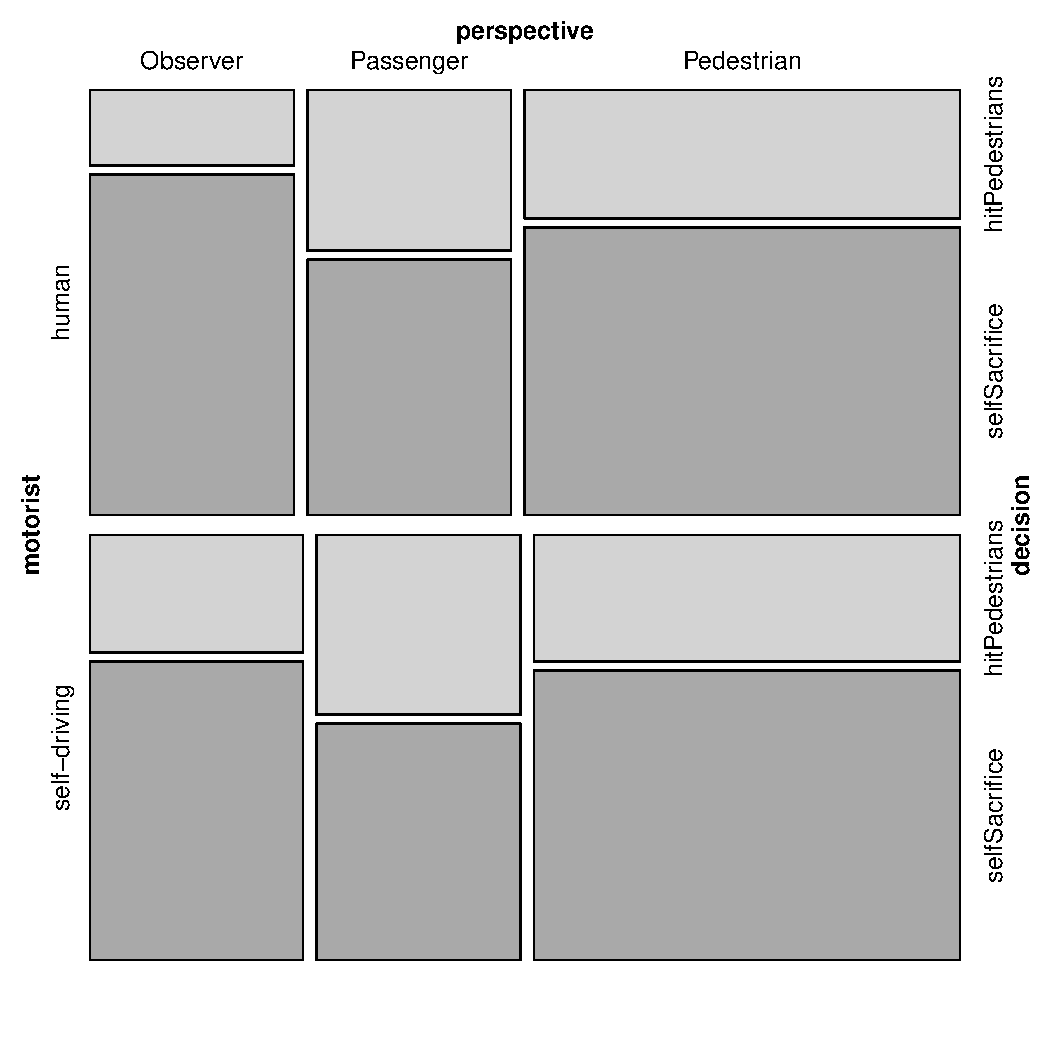
\includegraphics[width=\maxwidth]{figure/carsac-mosaic-1} 

\end{knitrout}

\subsection{The model}
\label{sec:carped-glmm}
\begin{kframe}
\begin{alltt}
\hlstd{(nc} \hlkwb{<-} \hlkwd{detectCores}\hlstd{())}
\end{alltt}
\end{kframe}[1] 12
\begin{kframe}\begin{alltt}
\hlstd{cl} \hlkwb{<-} \hlkwd{makeCluster}\hlstd{(}\hlkwd{rep}\hlstd{(}\hlstr{"localhost"}\hlstd{, nc))}

\hlstd{carsac_glmm} \hlkwb{<-} \hlkwd{mixed}\hlstd{(decision} \hlopt{~} \hlstd{perspective} \hlopt{+} \hlstd{motorist} \hlopt{+}
                        \hlstd{perspective}\hlopt{:}\hlstd{motorist} \hlopt{+}
                        \hlstd{trial} \hlopt{+} \hlstd{gender} \hlopt{+} \hlcom{#age +}
                        \hlstd{(}\hlnum{1} \hlopt{|} \hlstd{participant.ID),}
                    \hlkwc{method} \hlstd{=} \hlstr{"PB"}\hlstd{,} \hlcom{# change to PB for final}
                    \hlkwc{family} \hlstd{=} \hlstr{"binomial"}\hlstd{,} \hlkwc{data} \hlstd{= carsac.sub,}
                    \hlkwc{args_test} \hlstd{=} \hlkwd{list}\hlstd{(}\hlkwc{nsim} \hlstd{=} \hlnum{1000}\hlstd{,} \hlkwc{cl} \hlstd{= cl),} \hlkwc{cl} \hlstd{= cl,}
                    \hlkwc{control} \hlstd{=} \hlkwd{glmerControl}\hlstd{(}\hlkwc{optimizer} \hlstd{=} \hlstr{"bobyqa"}\hlstd{,}
                                           \hlkwc{optCtrl} \hlstd{=} \hlkwd{list}\hlstd{(}\hlkwc{maxfun} \hlstd{=} \hlnum{2e5}\hlstd{)))}
\end{alltt}


{\ttfamily\noindent\itshape\color{messagecolor}{\#\# Contrasts set to contr.sum for the following variables: decision, perspective, motorist, trial, gender, participant.ID}}\end{kframe}Fitting 6 (g)lmer() models.
Obtaining 5 p-values:
[.....]
\begin{kframe}\begin{alltt}
\hlkwd{stopCluster}\hlstd{(cl)}
\hlkwd{xtable}\hlstd{(carsac_glmm}\hlopt{$}\hlstd{anova_table)}
\end{alltt}
\end{kframe}% latex table generated in R 3.4.3 by xtable 1.8-2 package
% Wed Jan 24 19:48:51 2018
\begin{table}[ht]
\centering
\begin{tabular}{lrrrr}
  \hline
 & Chisq & Chi Df & Pr($>$Chisq) & Pr($>$PB) \\ 
  \hline
perspective & 7.50 & 2 & 0.0235 & 0.0311 \\ 
  motorist & 1.08 & 1 & 0.2994 & 0.3102 \\ 
  trial & 61.24 & 1 & 0.0000 & 0.0010 \\ 
  gender & 0.13 & 1 & 0.7228 & 0.7472 \\ 
  perspective:motorist & 1.05 & 2 & 0.5903 & 0.6148 \\ 
   \hline
\end{tabular}
\end{table}


Then we check the residuals.

\begin{knitrout}
\definecolor{shadecolor}{rgb}{0.969, 0.969, 0.969}\color{fgcolor}\begin{kframe}
\begin{alltt}
\hlstd{carsac_glmm.resid} \hlkwb{<-} \hlkwd{simulateResiduals}\hlstd{(}
    \hlkwc{fittedModel} \hlstd{= carsac_glmm}\hlopt{$}\hlstd{full_model,} \hlkwc{n} \hlstd{=} \hlnum{2000}\hlstd{)}
\hlstd{carsac_glmm_resid.plot} \hlkwb{<-} \hlkwd{plotSimulatedResiduals}\hlstd{(}
    \hlkwc{simulationOutput} \hlstd{= carsac_glmm.resid)}
\end{alltt}
\end{kframe}
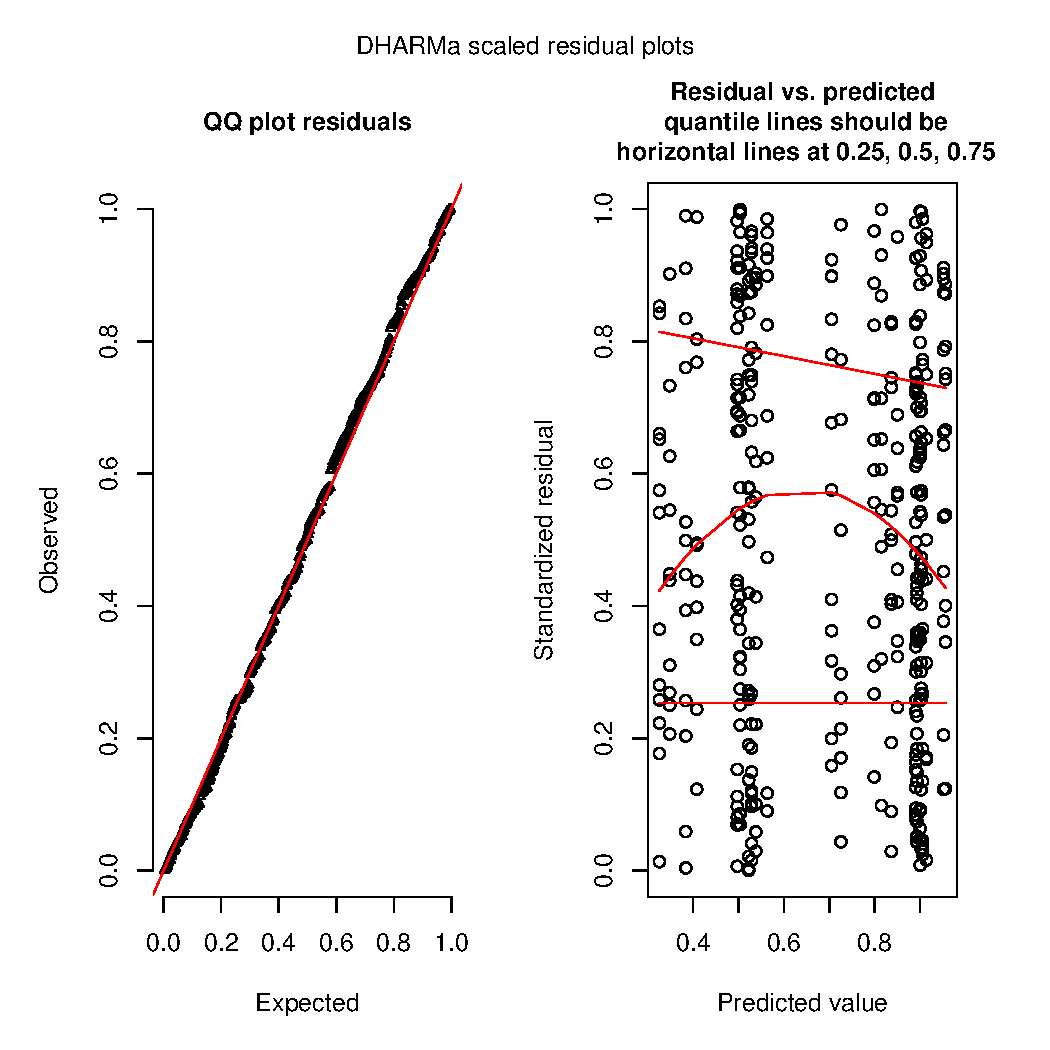
\includegraphics[width=\maxwidth]{figure/carped-resid-1} 

\end{knitrout}

\subsection{Plotting}
\label{sec:carped-plot}


Depending on which effects or interactions we find, we probably want to change this plot. It currently just plots the Estimated Marginal Means for the 2-way interaction.

\begin{knitrout}
\definecolor{shadecolor}{rgb}{0.969, 0.969, 0.969}\color{fgcolor}\begin{kframe}
\begin{alltt}
\hlstd{carsac.plot} \hlkwb{<-} \hlkwd{emmip}\hlstd{(carsac_glmm, perspective} \hlopt{~} \hlstd{trial} \hlopt{|} \hlstd{motorist,} \hlkwc{type} \hlstd{=} \hlstr{"response"}\hlstd{)} \hlopt{+}
    \hlkwd{theme_cowplot}\hlstd{(}\hlkwc{font_size} \hlstd{=} \hlnum{10}\hlstd{)} \hlopt{+}
    \hlkwd{scale_y_continuous}\hlstd{(}\hlkwc{name} \hlstd{=} \hlstr{"P(Choosing `crash car' as more acceptable)"}\hlstd{,}
                       \hlkwc{limits} \hlstd{=} \hlkwd{c}\hlstd{(}\hlnum{0}\hlstd{,} \hlnum{1}\hlstd{))} \hlopt{+} \hlkwd{coord_equal}\hlstd{(}\hlkwc{ratio} \hlstd{=} \hlnum{3}\hlstd{)} \hlopt{+}
    \hlkwd{scale_color_manual}\hlstd{(}\hlkwc{name} \hlstd{=} \hlstr{"Perspective"}\hlstd{,}
                       \hlkwc{labels} \hlstd{=} \hlkwd{c}\hlstd{(}\hlstr{"Bystander"}\hlstd{,}
                                  \hlstr{"Passenger"}\hlstd{,}
                                  \hlstr{"Pedestrian"}\hlstd{),}
                       \hlkwc{values} \hlstd{=} \hlkwd{c}\hlstd{(}\hlstr{"red3"}\hlstd{,} \hlstr{"skyblue"}\hlstd{,} \hlstr{"orange1"} \hlstd{,} \hlstr{"purple"}\hlstd{))}

\hlstd{carsac.plot}
\end{alltt}
\end{kframe}
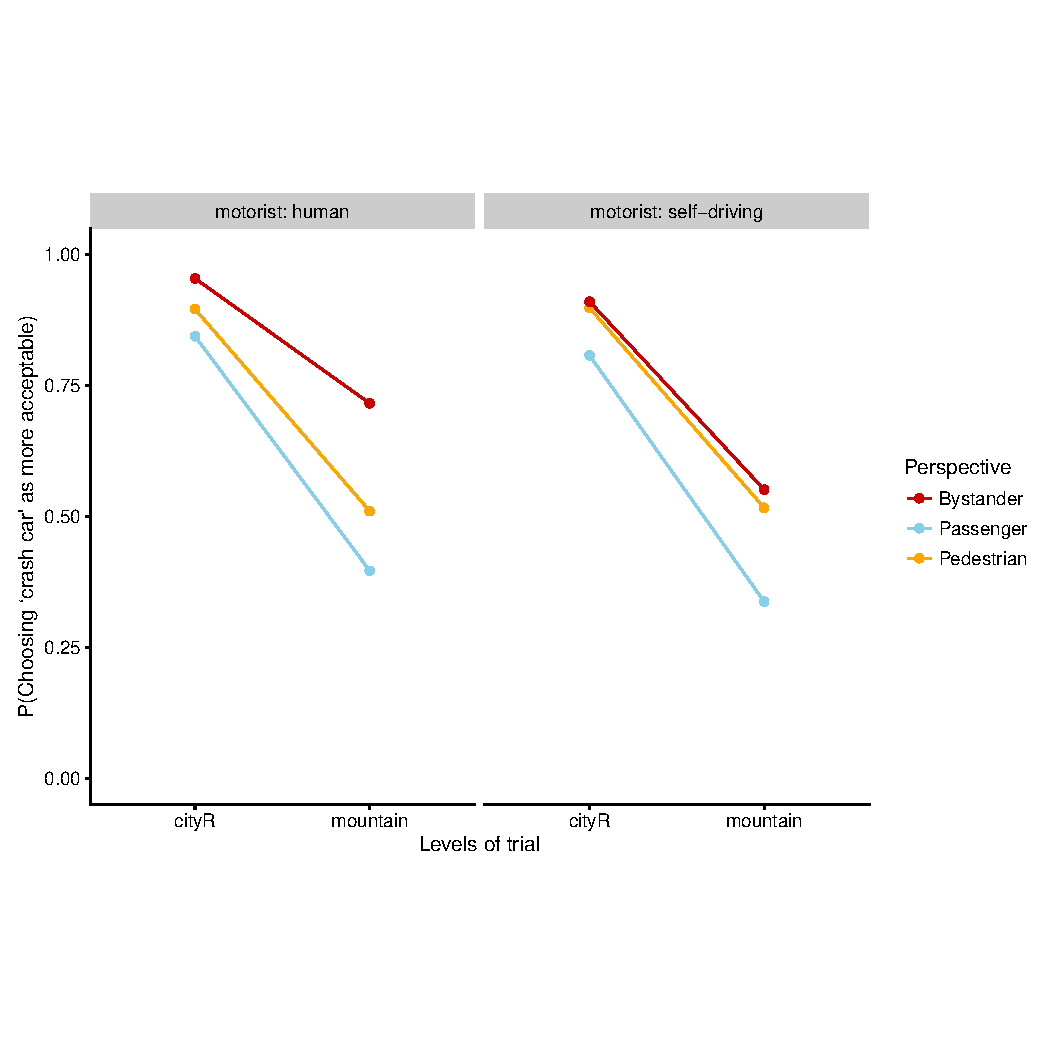
\includegraphics[width=\maxwidth]{figure/carped-plot-1} 

\end{knitrout}

\subsection{Follow-up analyses}
\label{sec:carped-followup}

If we find an interaction between perspective and motorist-type we
should follow that up with comparisons of perspective within each
level of motorist.

\begin{kframe}
\begin{alltt}
\hlstd{emm_carsac_i} \hlkwb{<-} \hlkwd{emmeans}\hlstd{(carsac_glmm, pairwise} \hlopt{~} \hlstd{perspective} \hlopt{|} \hlstd{motorist,}
                        \hlkwc{type} \hlstd{=} \hlstr{'response'}\hlstd{)}
\hlkwd{xtable}\hlstd{(emm_carsac_i}\hlopt{$}\hlstd{contrasts)}
\end{alltt}
\end{kframe}% latex table generated in R 3.4.3 by xtable 1.8-2 package
% Wed Jan 24 19:48:55 2018
\begin{table}[ht]
\centering
\begin{tabular}{lrrrrl}
  \hline
contrast & odds.ratio & SE & df & z.ratio & p.value \\ 
  \hline
\multicolumn{6}{l}{motorist = human}\\
Observer / Passenger & 3.8387 & 2.3773 & Inf & 2.172 & 0.0760 \\ 
  Observer / Pedestrian & 2.4179 & 1.3164 & Inf & 1.622 & 0.2364 \\ 
  Passenger / Pedestrian & 0.6299 & 0.3037 & Inf & -0.959 & 0.6032 \\ 
   \hline
\multicolumn{6}{l}{motorist = self-driving}\\
Observer / Passenger & 2.4128 & 1.3701 & Inf & 1.551 & 0.2672 \\ 
  Observer / Pedestrian & 1.1494 & 0.5673 & Inf & 0.282 & 0.9571 \\ 
  Passenger / Pedestrian & 0.4764 & 0.2310 & Inf & -1.529 & 0.2772 \\ 
   \hline
\multicolumn{6}{l}{{\footnotesize Results are averaged over the levels of: trial, gender}}\\

\multicolumn{6}{l}{{\footnotesize P value adjustment: tukey method for comparing a family of 3 estimates}}\\

\multicolumn{6}{l}{{\footnotesize Tests are performed on the log odds ratio scale}}\\
\end{tabular}
\end{table}


If we find no interaction but a significant main effect of
perspective, we need to do follow-up multiple comparisons to find out
where the difference is.

\begin{kframe}
\begin{alltt}
\hlstd{emm_carsac_persp} \hlkwb{<-} \hlkwd{emmeans}\hlstd{(carsac_glmm, pairwise} \hlopt{~} \hlstd{perspective,}
                            \hlkwc{type} \hlstd{=} \hlstr{'response'}\hlstd{)}
\end{alltt}


{\ttfamily\noindent\itshape\color{messagecolor}{\#\# NOTE: Results may be misleading due to involvement in interactions}}\begin{alltt}
\hlkwd{xtable}\hlstd{(emm_carsac_persp}\hlopt{$}\hlstd{contrasts)}
\end{alltt}
\end{kframe}% latex table generated in R 3.4.3 by xtable 1.8-2 package
% Wed Jan 24 19:48:55 2018
\begin{table}[ht]
\centering
\begin{tabular}{lrrrrl}
  \hline
contrast & odds.ratio & SE & df & z.ratio & p.value \\ 
  \hline
Observer / Passenger & 3.0433 & 1.3025 & Inf & 2.600 & 0.0252 \\ 
  Observer / Pedestrian & 1.6671 & 0.6142 & Inf & 1.387 & 0.3475 \\ 
  Passenger / Pedestrian & 0.5478 & 0.1889 & Inf & -1.745 & 0.1885 \\ 
   \hline
\multicolumn{6}{l}{{\footnotesize Results are averaged over the levels of: motorist, trial, gender}}\\

\multicolumn{6}{l}{{\footnotesize P value adjustment: tukey method for comparing a family of 3 estimates}}\\

\multicolumn{6}{l}{{\footnotesize Tests are performed on the log odds ratio scale}}\\
\end{tabular}
\end{table}


If we find a main effect of motorist-type, we need to calculate the
marginal means to see the effect.

\begin{kframe}
\begin{alltt}
\hlstd{emm_carsac_motorist} \hlkwb{<-} \hlkwd{emmeans}\hlstd{(carsac_glmm, pairwise} \hlopt{~} \hlstd{motorist,}
                               \hlkwc{type} \hlstd{=} \hlstr{'response'}\hlstd{)}
\end{alltt}


{\ttfamily\noindent\itshape\color{messagecolor}{\#\# NOTE: Results may be misleading due to involvement in interactions}}\begin{alltt}
\hlkwd{xtable}\hlstd{(emm_carsac_motorist}\hlopt{$}\hlstd{contrasts)}
\end{alltt}
\end{kframe}% latex table generated in R 3.4.3 by xtable 1.8-2 package
% Wed Jan 24 19:48:55 2018
\begin{table}[ht]
\centering
\begin{tabular}{lrrrrl}
  \hline
contrast & odds.ratio & SE & df & z.ratio & p.value \\ 
  \hline
human / self-driving & 1.3710 & 0.4191 & Inf & 1.032 & 0.3020 \\ 
   \hline
\multicolumn{6}{l}{{\footnotesize Results are averaged over the levels of: perspective, trial, gender}}\\

\multicolumn{6}{l}{{\footnotesize Tests are performed on the log odds ratio scale}}\\
\end{tabular}
\end{table}


\section{Sidewalk vs road dilemma}
\label{sec:sidewalk}

\begin{knitrout}
\definecolor{shadecolor}{rgb}{0.969, 0.969, 0.969}\color{fgcolor}\begin{kframe}
\begin{alltt}
\hlstd{sidewalk.xtabs} \hlkwb{<-} \hlkwd{xtabs}\hlstd{(}\hlopt{~} \hlstd{motorist} \hlopt{+} \hlstd{perspective} \hlopt{+} \hlstd{decision,} \hlkwc{data} \hlstd{= sidewalk.sub)}
\hlstd{sidewalk.mosaic} \hlkwb{<-} \hlkwd{mosaic}\hlstd{(sidewalk.xtabs,}
                       \hlkwc{gp} \hlstd{=} \hlkwd{gpar}\hlstd{(}\hlkwc{fill} \hlstd{=} \hlkwd{c}\hlstd{(}\hlstr{"light gray"}\hlstd{,} \hlstr{"dark gray"}\hlstd{)))}
\end{alltt}
\end{kframe}
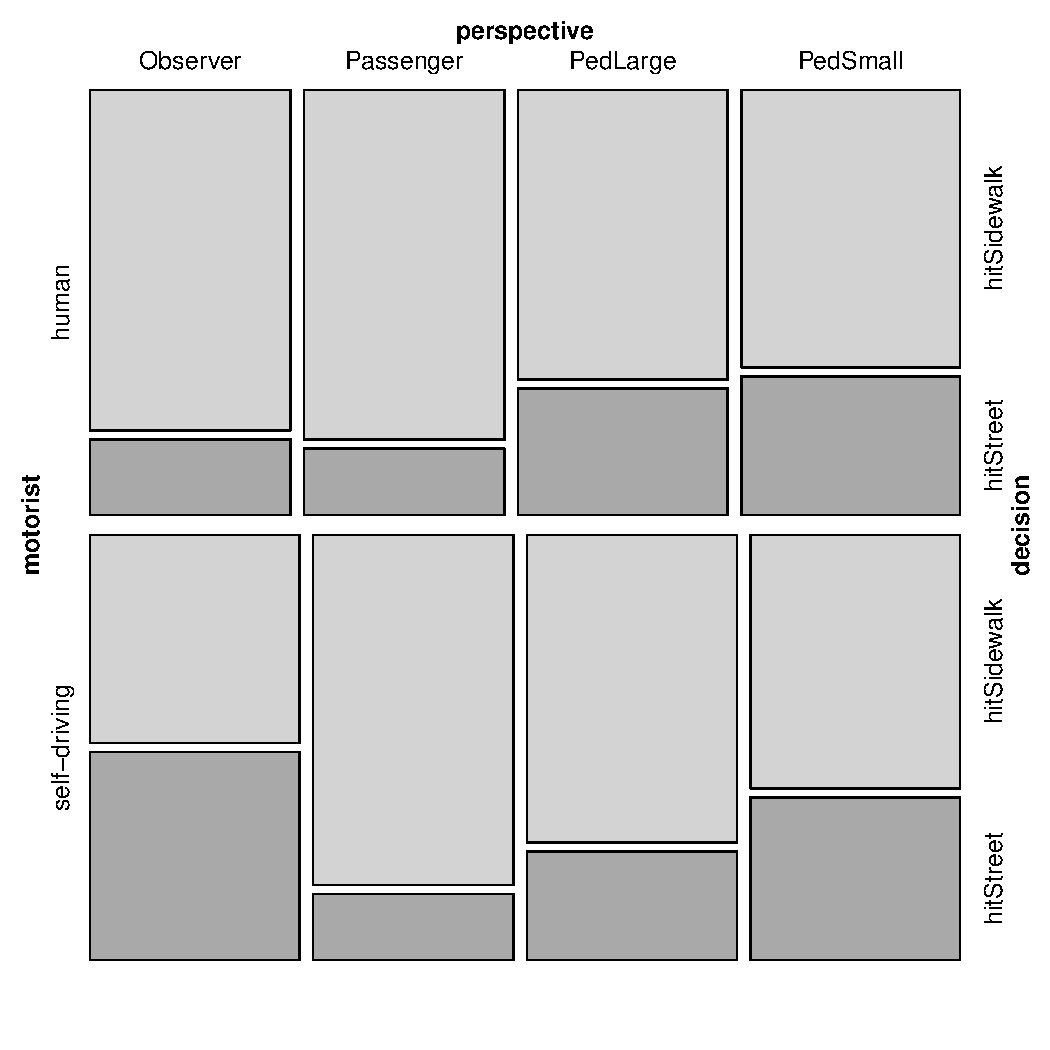
\includegraphics[width=\maxwidth]{figure/sidewalk-mosaic-1} 

\end{knitrout}

\subsection{The model}
\label{sec:sidewalk-glmm}
\begin{kframe}
\begin{alltt}
\hlstd{(nc} \hlkwb{<-} \hlkwd{detectCores}\hlstd{())}
\end{alltt}
\end{kframe}[1] 12
\begin{kframe}\begin{alltt}
\hlstd{cl} \hlkwb{<-} \hlkwd{makeCluster}\hlstd{(}\hlkwd{rep}\hlstd{(}\hlstr{"localhost"}\hlstd{, nc))}

\hlstd{sidewalk_glmm} \hlkwb{<-} \hlkwd{mixed}\hlstd{(decision} \hlopt{==} \hlstr{'hitSidewalk'} \hlopt{~} \hlstd{perspective} \hlopt{+}
                        \hlstd{motorist} \hlopt{+}
                        \hlstd{perspective}\hlopt{:}\hlstd{motorist} \hlopt{+}
                        \hlstd{trial} \hlopt{+} \hlstd{gender} \hlopt{+} \hlcom{#age +}
                        \hlstd{(}\hlnum{1} \hlopt{|} \hlstd{participant.ID),}
                    \hlkwc{method} \hlstd{=} \hlstr{"PB"}\hlstd{,} \hlcom{# change to PB for final}
                    \hlkwc{family} \hlstd{=} \hlstr{"binomial"}\hlstd{,} \hlkwc{data} \hlstd{= sidewalk.sub,}
                    \hlkwc{args_test} \hlstd{=} \hlkwd{list}\hlstd{(}\hlkwc{nsim} \hlstd{=} \hlnum{1000}\hlstd{,} \hlkwc{cl} \hlstd{= cl),} \hlkwc{cl} \hlstd{= cl,}
                    \hlkwc{control} \hlstd{=} \hlkwd{glmerControl}\hlstd{(}\hlkwc{optimizer} \hlstd{=} \hlstr{"bobyqa"}\hlstd{,}
                                           \hlkwc{optCtrl} \hlstd{=} \hlkwd{list}\hlstd{(}\hlkwc{maxfun} \hlstd{=} \hlnum{2e5}\hlstd{)))}
\end{alltt}


{\ttfamily\noindent\itshape\color{messagecolor}{\#\# Contrasts set to contr.sum for the following variables: decision, perspective, motorist, trial, gender, participant.ID}}\end{kframe}Fitting 6 (g)lmer() models.
Obtaining 5 p-values:
[.....]
\begin{kframe}\begin{alltt}
\hlkwd{stopCluster}\hlstd{(cl)}
\hlkwd{xtable}\hlstd{(sidewalk_glmm}\hlopt{$}\hlstd{anova_table)}
\end{alltt}
\end{kframe}% latex table generated in R 3.4.3 by xtable 1.8-2 package
% Wed Jan 24 20:15:31 2018
\begin{table}[ht]
\centering
\begin{tabular}{lrrrr}
  \hline
 & Chisq & Chi Df & Pr($>$Chisq) & Pr($>$PB) \\ 
  \hline
perspective & 7.93 & 3 & 0.0475 & 0.0526 \\ 
  motorist & 2.12 & 1 & 0.1455 & 0.2086 \\ 
  trial & 4.00 & 1 & 0.0455 & 0.0909 \\ 
  gender & 4.90 & 1 & 0.0268 & 0.0058 \\ 
  perspective:motorist & 6.64 & 3 & 0.0842 & 0.0536 \\ 
   \hline
\end{tabular}
\end{table}


Then we check the residuals.

\begin{knitrout}
\definecolor{shadecolor}{rgb}{0.969, 0.969, 0.969}\color{fgcolor}\begin{kframe}
\begin{alltt}
\hlstd{sidewalk_glmm.resid} \hlkwb{<-} \hlkwd{simulateResiduals}\hlstd{(}
    \hlkwc{fittedModel} \hlstd{= sidewalk_glmm}\hlopt{$}\hlstd{full_model,} \hlkwc{n} \hlstd{=} \hlnum{2000}\hlstd{)}
\hlstd{sidewalk_glmm_resid.plot} \hlkwb{<-} \hlkwd{plotSimulatedResiduals}\hlstd{(}
    \hlkwc{simulationOutput} \hlstd{= sidewalk_glmm.resid)}
\end{alltt}
\end{kframe}
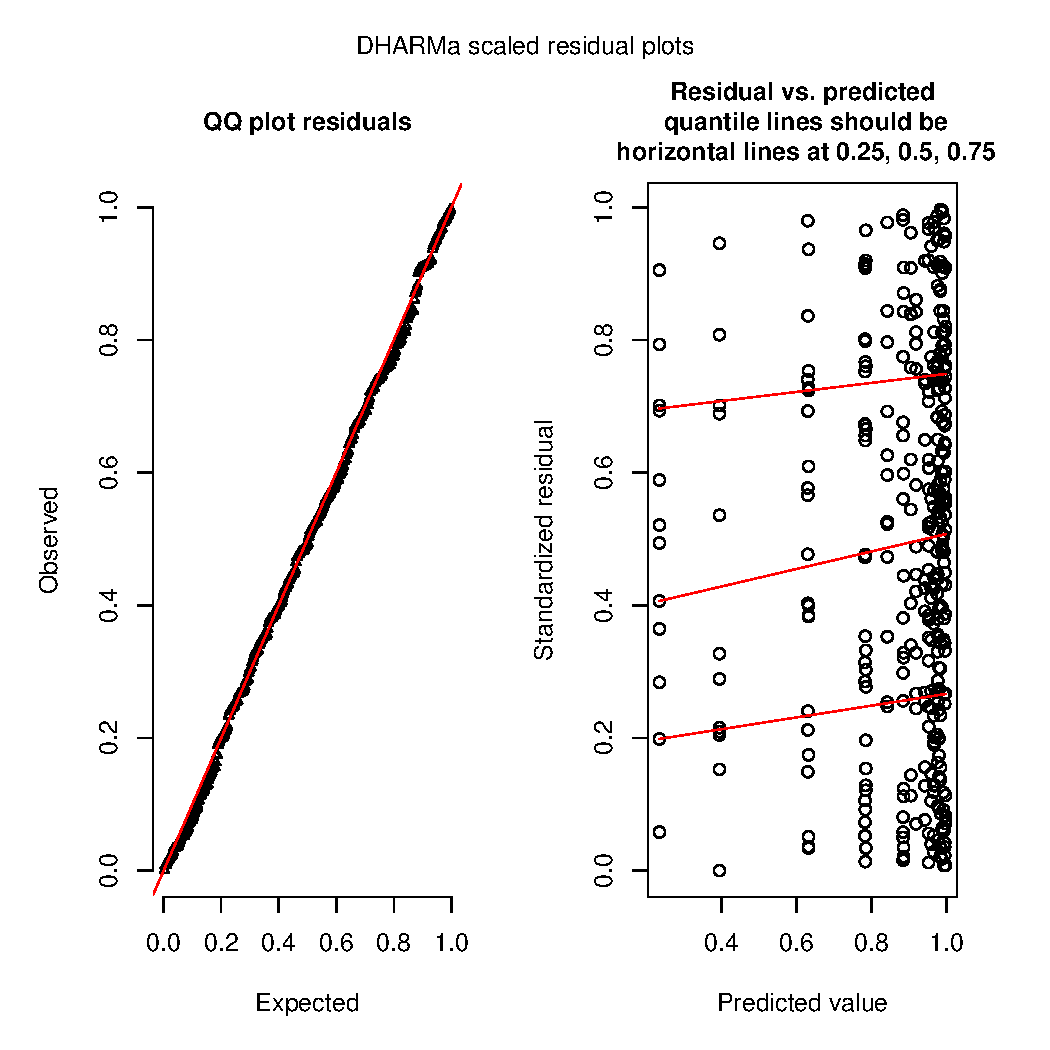
\includegraphics[width=\maxwidth]{figure/sidewalk-resid-1} 

\end{knitrout}

\subsection{Plotting}
\label{sec:sidewalk-plot}

Depending on which effects or interactions we find, we probably want to change this plot. It currently just plots the Estimated Marginal Means for the 2-way interaction.

\begin{knitrout}
\definecolor{shadecolor}{rgb}{0.969, 0.969, 0.969}\color{fgcolor}\begin{kframe}
\begin{alltt}
\hlstd{sidewalk.plot} \hlkwb{<-} \hlkwd{emmip}\hlstd{(sidewalk_glmm, perspective} \hlopt{~} \hlstd{trial} \hlopt{|} \hlstd{motorist,}
                       \hlkwc{type} \hlstd{=} \hlstr{"response"}\hlstd{)} \hlopt{+}
    \hlkwd{theme_cowplot}\hlstd{(}\hlkwc{font_size} \hlstd{=} \hlnum{10}\hlstd{)} \hlopt{+}
    \hlkwd{scale_y_continuous}\hlstd{(}
        \hlkwc{name} \hlstd{=} \hlstr{"P(Choosing `swerve to sidewalk' as more acceptable)"}\hlstd{,}
                       \hlkwc{limits} \hlstd{=} \hlkwd{c}\hlstd{(}\hlnum{0}\hlstd{,} \hlnum{1}\hlstd{))} \hlopt{+} \hlkwd{coord_equal}\hlstd{(}\hlkwc{ratio} \hlstd{=} \hlnum{3}\hlstd{)} \hlopt{+}
    \hlkwd{scale_color_manual}\hlstd{(}\hlkwc{name} \hlstd{=} \hlstr{"Perspective"}\hlstd{,}
                       \hlkwc{labels} \hlstd{=} \hlkwd{c}\hlstd{(}\hlstr{"Bystander"}\hlstd{,}
                                  \hlstr{"Passenger"}\hlstd{,}
                                  \hlstr{"Pedestrian on road"}\hlstd{,}
                                  \hlstr{"Pedestrian on sidewalk"}\hlstd{),}
                       \hlkwc{values} \hlstd{=} \hlkwd{c}\hlstd{(}\hlstr{"red3"}\hlstd{,} \hlstr{"skyblue"}\hlstd{,}
                                  \hlstr{"orange1"}\hlstd{,} \hlstr{"purple"}\hlstd{))}

\hlstd{sidewalk.plot}
\end{alltt}
\end{kframe}
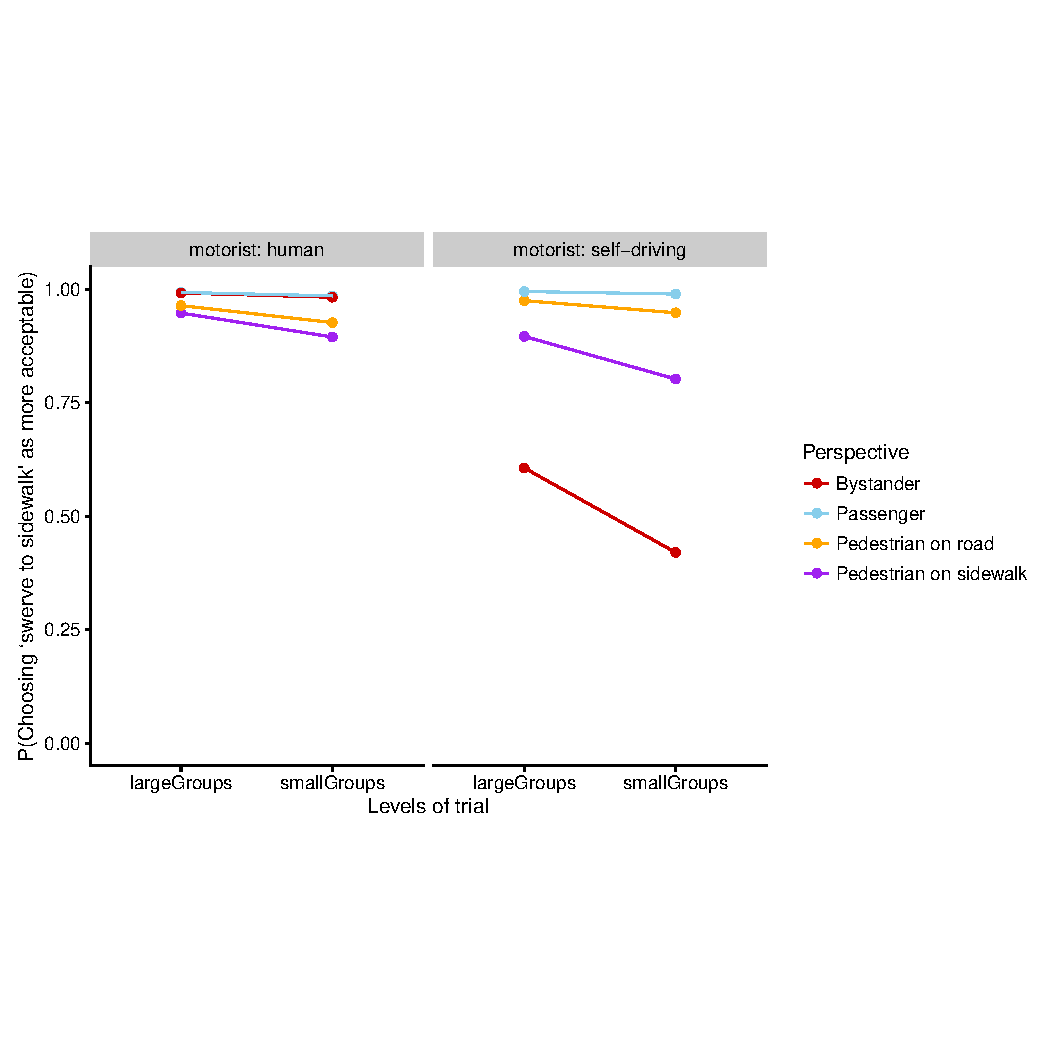
\includegraphics[width=\maxwidth]{figure/sidewalk-plot-1} 

\end{knitrout}

\subsection{Follow-up analyses}
\label{sec:sidewalk-followup}

If we find an interaction between perspective and motorist-type we
should follow that up with comparisons of perspective within each
level of motorist.

\begin{kframe}
\begin{alltt}
\hlstd{emm_sidewalk_i} \hlkwb{<-} \hlkwd{emmeans}\hlstd{(sidewalk_glmm, pairwise} \hlopt{~} \hlstd{perspective} \hlopt{|} \hlstd{motorist,}
                          \hlkwc{type} \hlstd{=} \hlstr{'response'}\hlstd{)}
\hlkwd{xtable}\hlstd{(emm_sidewalk_i}\hlopt{$}\hlstd{contrasts)}
\end{alltt}
\end{kframe}% latex table generated in R 3.4.3 by xtable 1.8-2 package
% Wed Jan 24 20:15:34 2018
\begin{table}[ht]
\centering
\begin{tabular}{lrrrrl}
  \hline
contrast & odds.ratio & SE & df & z.ratio & p.value \\ 
  \hline
\multicolumn{6}{l}{motorist = human}\\
Observer / Passenger & 0.8300 & 1.1971 & Inf & 0.693 & 0.8997 \\ 
  Observer / PedLarge & 4.4380 & 6.5893 & Inf & 0.674 & 0.9071 \\ 
  Observer / PedSmall & 6.5827 & 9.7895 & Inf & 0.672 & 0.9075 \\ 
  Passenger / PedLarge & 5.3471 & 7.9321 & Inf & 0.674 & 0.9069 \\ 
  Passenger / PedSmall & 7.9310 & 11.7982 & Inf & 0.672 & 0.9076 \\ 
  PedLarge / PedSmall & 1.4832 & 2.2475 & Inf & 0.660 & 0.9121 \\ 
   \hline
\multicolumn{6}{l}{motorist = self-driving}\\
Observer / Passenger & 0.0077 & 0.0151 & Inf & 0.510 & 0.9568 \\ 
  Observer / PedLarge & 0.0395 & 0.0721 & Inf & 0.549 & 0.9469 \\ 
  Observer / PedSmall & 0.1785 & 0.3171 & Inf & 0.563 & 0.9430 \\ 
  Passenger / PedLarge & 5.1422 & 7.5438 & Inf & 0.682 & 0.9041 \\ 
  Passenger / PedSmall & 23.2135 & 37.5966 & Inf & 0.617 & 0.9266 \\ 
  PedLarge / PedSmall & 4.5143 & 7.0392 & Inf & 0.641 & 0.9186 \\ 
   \hline
\multicolumn{6}{l}{{\footnotesize Results are averaged over the levels of: trial, gender}}\\

\multicolumn{6}{l}{{\footnotesize Unknown transformation "==": no transformation done}}\\

\multicolumn{6}{l}{{\footnotesize P value adjustment: tukey method for comparing a family of 4 estimates}}\\
\end{tabular}
\end{table}


If we find no interaction but a significant main effect of
perspective, we need to do follow-up multiple comparisons to find out
where the difference is.

\begin{kframe}
\begin{alltt}
\hlstd{emm_sidewalk_persp} \hlkwb{<-} \hlkwd{emmeans}\hlstd{(sidewalk_glmm, pairwise} \hlopt{~} \hlstd{perspective,}
                              \hlkwc{type} \hlstd{=} \hlstr{'response'}\hlstd{)}
\end{alltt}


{\ttfamily\noindent\itshape\color{messagecolor}{\#\# NOTE: Results may be misleading due to involvement in interactions}}\begin{alltt}
\hlkwd{xtable}\hlstd{(emm_sidewalk_persp}\hlopt{$}\hlstd{contrasts)}
\end{alltt}
\end{kframe}% latex table generated in R 3.4.3 by xtable 1.8-2 package
% Wed Jan 24 20:15:34 2018
\begin{table}[ht]
\centering
\begin{tabular}{lrrrrl}
  \hline
contrast & odds.ratio & SE & df & z.ratio & p.value \\ 
  \hline
Observer / Passenger & 0.0799 & 0.0977 & Inf & 0.818 & 0.8462 \\ 
  Observer / PedLarge & 0.4189 & 0.4855 & Inf & 0.863 & 0.8240 \\ 
  Observer / PedSmall & 1.0841 & 1.2186 & Inf & 0.890 & 0.8103 \\ 
  Passenger / PedLarge & 5.2436 & 5.5014 & Inf & 0.953 & 0.7760 \\ 
  Passenger / PedSmall & 13.5686 & 15.2436 & Inf & 0.890 & 0.8100 \\ 
  PedLarge / PedSmall & 2.5876 & 2.8321 & Inf & 0.914 & 0.7976 \\ 
   \hline
\multicolumn{6}{l}{{\footnotesize Results are averaged over the levels of: motorist, trial, gender}}\\

\multicolumn{6}{l}{{\footnotesize Unknown transformation "==": no transformation done}}\\

\multicolumn{6}{l}{{\footnotesize P value adjustment: tukey method for comparing a family of 4 estimates}}\\
\end{tabular}
\end{table}


If we find a main effect of motorist-type, we need to calculate the
marginal means to see the effect.

\begin{kframe}
\begin{alltt}
\hlstd{emm_sidewalk_motorist} \hlkwb{<-} \hlkwd{emmeans}\hlstd{(sidewalk_glmm, pairwise} \hlopt{~} \hlstd{motorist,}
                                 \hlkwc{type} \hlstd{=} \hlstr{'response'}\hlstd{)}
\end{alltt}


{\ttfamily\noindent\itshape\color{messagecolor}{\#\# NOTE: Results may be misleading due to involvement in interactions}}\begin{alltt}
\hlkwd{xtable}\hlstd{(emm_sidewalk_motorist}\hlopt{$}\hlstd{contrasts)}
\end{alltt}
\end{kframe}% latex table generated in R 3.4.3 by xtable 1.8-2 package
% Wed Jan 24 20:15:34 2018
\begin{table}[ht]
\centering
\begin{tabular}{lrrrrl}
  \hline
contrast & odds.ratio & SE & df & z.ratio & p.value \\ 
  \hline
human / self-driving & 2.9910 & 2.4391 & Inf & 1.226 & 0.2201 \\ 
   \hline
\multicolumn{6}{l}{{\footnotesize Results are averaged over the levels of: perspective, trial, gender}}\\

\multicolumn{6}{l}{{\footnotesize Unknown transformation "==": no transformation done}}\\
\end{tabular}
\end{table}





\end{document}
